\documentclass{article}
\usepackage[utf8]{inputenc}
\usepackage{amsfonts,amssymb}
\usepackage[fleqn]{amsmath}
\usepackage{bm}
\usepackage{graphicx}
\usepackage{epstopdf}
\usepackage{color}
\usepackage{enumitem}
\usepackage{listings}
\usepackage{appendix}
\usepackage{hyperref}


\title{Report of EE6483 project}
\author{ Li siqi, Yang kaiwen, Zheng zhikai}
\begin{document}



\maketitle
\section{Notice}

This project was collaboratively completed by a team of three students: LI SIQI, YANG KAIWEN, and ZHENG ZHIKAI. As per the project requirements, the division of tasks among the team members is detailed in \hyperlink{apdxA}{Appendix A}. The project's relevant code has been hosted on GitHub at \url{https://github.com/KuRRe8/Bi-Senti-EE6483} . The repository will be made public at 12:00 AM on November 16, 2024. All implementation methods discussed in this report are included in the repository files. However, due to file size limitations, the fine-tuned model has not been uploaded to GitHub. If verification is needed, please contact the team members.

\section{Intro}

\hypertarget{hpa.1}{{\color{red}{\hyperlink{hhpa.1}{task a.1}}}} Sentiment Analysis, also known as Opinion Mining, is one of the most important tasks in the field of natural language processing (NLP). Sentiment Analysis aims to analyze text data and determine its sentiment (positive, neutral, or negative). It is widely used in e-commerce, social media monitoring, and market research. For example, by analyzing user reviews of products, companies can better understand customer needs and improve their product strategies. In social media, sentiment analysis can be used to track the public's attitudes towards events and predict trends. As user-generated content (UGC) continues to grow, the demand for sentiment analysis is increasing, and its research has gradually become a hotspot in the field of NLP research.

The task of sentiment analysis faces many challenges, mainly in the following aspects:
 
 1.Sparse and diverse data: User-generated text often contains spelling errors, informal expressions, and polysemous words, which makes it difficult to understand the semantics of the text.
 
 2.Capturing contextual information: Emotional expressions are often dependent on context, while traditional Bag-of-Words or TF-IDF {\color{blue}{[1]}} methods are unable to effectively capture the sequential information and contextual relationships in the text.
 
 3.Implicit emotional expression: Some text's emotional expression may be subtle, such as sarcastic language, which increase the requirements of the model's ability to identify emotions.

To address these challenges, the field of sentiment analysis has gradually evolved from traditional machine learning methods to deep learning techniques. These methods have significantly improved in feature extraction, semantic understanding, and context capturing capabilities. The goal of this project is to classify the sentiment of given comment data sets using a combination of existing machine learning and deep learning methods, and to determine the sentiment polarity (positive, neutral, or negative) of each comment. We used a variety of methods, including traditional methods such as TF-IDF {\color{blue}{[1]}} and support vector machines (SVM){\color{blue}{[2]}}{\color{blue}{[3]}}{\color{blue}{[4]}}, and deep learning methods such as classifiers based on recurrent neural networks (RNN) {\color{blue}{[5]}}{\color{blue}{[6]}}, long short-term memory networks (LSTM) {\color{blue}{[7]}}{\color{blue}{[8]}}, and pre-trained models (BERT) {\color{blue}{[9]}}. Through the implementation of these methods, we modeled and predicted the training and test sets of the data set, and determined the sentiment polarity of each comment (positive, neutral, or negative).

\section{Related work}

\hypertarget{hpa.2}{{\color{red}{\hyperlink{hhpa.2}{task a.2}}}}In the early studies of sentiment analysis, traditional machine learning methods dominated. The core process of these methods includes two stages: first, converting text into numerical representation through explicit feature engineering; then, completing the sentiment classification task using classical classifiers. In terms of text feature extraction, TF-IDF and Bag-of-Words are the most used methods. They can convert text into a vector representation of fixed dimension, thus providing input for subsequent classifiers. However, the limitations of these methods lie in their inability to capture the semantic relationships between words and the contextual information of the text, thus limiting their ability to handle complex semantics. In terms of classifier selection, support vector machines (SVM) were the preferred model for early sentiment analysis due to their stable performance on small-scale data sets. In addition, random forests {\color{blue}{[4]}}{\color{blue}{[10]}} and Gaussian processes {\color{blue}{[11]}}{\color{blue}{[12]}} were widely used in specific scenarios. These models have certain advantages in computational efficiency and implementation difficulty, but as the task complexity increases, they gradually reveal their shortcomings in capturing deep-level semantics and handling large-scale data.

With the introduction of text embedding methods, sentiment analysis tasks gradually shifted from simple feature engineering to semantic modeling. Static embedding methods, such as Word2Vec {\color{blue}{[13]}}, FastText {\color{blue}{[14]}}{\color{blue}{[15]}}{\color{blue}{[16]}}, and GloVe {\color{blue}{[17]}}, can capture the semantic relationships of words through vector representations and significantly improve the quality of text representation. However, these methods lack sensitivity to context and are difficult to handle the problem of polysemy of the same word in different contexts. In contrast, dynamic embedding methods (such as BERT {\color{blue}{[9]}}) greatly improve the semantic understanding ability of text by generating different vector representations for the same word in different contexts.

\hypertarget{hpa.3}{{\color{red}{\hyperlink{hhpa.3}{task a.3}}}}With the rapid development of deep learning, neural network-based methods have gradually replaced traditional methods and become the mainstream technology for sentiment analysis. These methods can automatically extract features and capture contextual semantic information through end-to-end learning. Recurrent neural networks (RNN){\color{blue}{[5]}}{\color{blue}{[6]}}: RNN captures the sequential dependencies in text through its recurrent structure, making it one of the earliest deep learning models applied in sentiment analysis. However, RNN has the problem of gradient vanishing, limiting its performance in long text analysis. Long short-term memory networks (LSTM) {\color{blue}{[7]}}{\color{blue}{[8]}}: LSTM effectively solves the gradient problem of RNN by introducing a memory gate mechanism, becoming a popular choice for text sentiment analysis. In recent years, BERT {\color{blue}{[9]}} and its related models such as Roberta {\color{blue}{[18]}}, DistilBert {\color{blue}{[19]}}, and Albert {\color{blue}{[20]}}, which are pre-trained language models based on Transformer, have performed well in sentiment analysis with their strong context modeling ability and cross-task adaptability. These models can learn rich semantic information from large-scale pre-training corpora and fine-tune themselves for specific tasks. 

Recent large language models (LLMs) such as OpenAI's GPT series and Google's PaLM series have made significant progress. These models not only have strong generation and comprehension abilities but also can perform well in sentiment classification tasks with zero-shot and few-shot learning. Brown et al. {\color{blue}{[21]}} proposed GPT-3 model, which achieved efficient modeling of sentiment analysis tasks through prompt engineering, avoiding complicated fine-tuning steps. Ouyang et al. 's InstructGPT {\color{blue}{[22]}} further optimized the model performance by combining human feedback, reaching a new height in flexibility and controllability. Compared with traditional pre-trained models such as BERT, these large language models have significant advantages in context capture, polysemy handling, and task generalization ability, providing more efficient and convenient solutions for sentiment analysis tasks.

\hypertarget{hpa.4}{{\color{red}{\hyperlink{hhpa.4}{task a.4}}}}Fine-tuning a pre-trained BERT model is a suitable baseline for sentiment binary classification of product reviews due to its strong contextual understanding and pre-training on large corpora. BERT effectively captures the nuances in text, such as the contextual meaning of words, making it ideal for this task. To implement this solution, we should fine-tune BERT on a domain-specific dataset of product reviews, ensuring the model adapts to the language and patterns of the target domain. Optimizing the tokenizer to handle product-specific terms can further enhance performance. If the dataset is imbalanced, applying techniques like weighted loss functions or data augmentation can address this issue. Additionally, hyperparameter tuning, such as adjusting the learning rate or batch size, is essential for maximizing performance. Finally, incorporating post-processing techniques like attention visualization can improve interpretability, building trust in the model's predictions. This approach balances simplicity and effectiveness, leveraging BERT’s strengths for the task.

\section{Experimental Design}
From this part, we will focus on our code implementation. Our goal is to design a flexible program that \textbf{can freely combine substeps} to utilize most popular methods. These substeps include: 

Reading in data (Pandas), Preprocessing (Regular Expression, Tokenize, Stop words, Lemmatization), Embedding (Word2Vec, GloVe, FastText, TF-IDF, Context-based Embedding), Model Selection (Support Vector Machine, Extreme Learning Machine, Gaussian Process, RNN, LSTM, GRU, BERT/DistilBERT/Roberta), Training (Sci-kit learn, PyTorch, Transformer (HuggingFace), Optuna, Ray Tune), Evaluate and Prediction (Accuracy, F1-score)


\subsection{Preprocessing}
The raw text needs to be processed before being put into the model. 

In non-huggingface routine, we first use RegEx to remove punctuation. Then there are 3 choices to use to tokenize the "str" type text, namely nltk.tokenize.word\_tokenize(), spacy.Language.doc.tokens.text, gensim.utils.simple\_preprocess(), after this step, our training data should be this type list[list[str]].

After that we provide multiple ways to remove stop words. Stop words are most common words in English that does not provide meaningful context. \\Lemmatization is also a significant step to process, this method will give the original form of a word, this is especially useful in English. In detail, we first use nktl.pos\_tag() to get the "part of speech" information, and then use this information to get the origin form of words.

Now we still have the data in list[list[str]], we should convert them into numerical representation, embedding. We introduced many popular methods to deal with the word embeddings. Word2Vec is a shallow neural network proposed by Google. It contains 2 ways to get embeddings, CBOW and Skip-gram. Here we can train our own Word2Vec model or just use pretrained GoogleNews-vectors-negative300.bin. Another approach is to use Glove model by pretrained glove-wiki-gigaword-100. \hypertarget{hpb}{{\color{red}{\hyperlink{hhpb}{task b}}}}In this step, our data will be transformed to the type of list[list[list[float64]]], if we use google embedding, the shape is 7401*words*300. There are 7401 training samples in train.json, in each sentence, the words count is different, and for each word, there are 300 float number to represent it.

TF-IDF is a BOW method, it calculate the frequency and inverse frequency, finally the whole sentence will transformed to a vector. This operation will lose the sequence infomation, so in our code, TF-IDF method is not encouraged.

In huggingface finetune routine, most of the preprocessing are automatically done. We could simply use AutoTokenizer.from\_pretrained() to load official tokenizer or our finetuned model tokenizer. Warp the input data to Dataset and apply the tokenizer, finally we will get the dict representing a sentence:\\input\_ids: a tensor with shape [1,128] since we explicitly constrain the sentence length to 128(if shorter, padding it), input\_ids is the id of token. \\attention\_mask: it is 1 if current position is a real word, 0 if it is padding. Of course the shape of tensor is same to input\_ids [1,128]\\token\_type\_ids: it is used to differentiate the sentence A and sentence B.

\subsection{Model Selection}

Since this is a programming scene, we have classified the model into three categories based on the software library. (All of the methods mentioned later are already implemented in code)
\begin{enumerate}
    \item Sci-kit learn: Traditional machine learning based classifiers. These classifiers are estimators for general use, SVM/ ELM/ GP. We can just put our numerical data and the label into the model. The best practice of Sci-kit learn is to use the GridSearch, it combines hyperparameter search algorithm, the pipeline and the cross validation such as Kfold.
    \item Pytorch: Provides deep learning essential blocks. We can use Torch to construct our customized RNN/ LSTM/ GRU. In this scenario, we often add a linear layer with 1 output neuron for binary sentiment classification. Here we use OptunaSearch to find the best hyperparameters.
    \item Transformer: It is a lib by HuggingFace. In this task, we will talk more details of Bert pretrained model using Transformer lib.
\end{enumerate}

We have finetuned 3 encoder-only model, Bert/ DistilBert/ Roberta. Bert was first proposed in 2018, DistilBERT compresses the model using knowledge distillation, increasing training speed with minimal performance loss on downstream tasks. In contrast, RoBERTa uses more training data, removes the Next Sentence Prediction (NSP) task, and generates masks dynamically. \hypertarget{hpc}{{\color{red}{\hyperlink{hhpc}{task c}}}}Here, we primarily focus on the details of using BERT.

After the preprocessing step, we convert the sentence into dict\{input\_ids, attention\_mask, token\_type\_ids\} as shown in Figure \ref{fig:input}, for this case, the shape is 128+128+128 for one sentence.

\begin{figure}
    \centering
    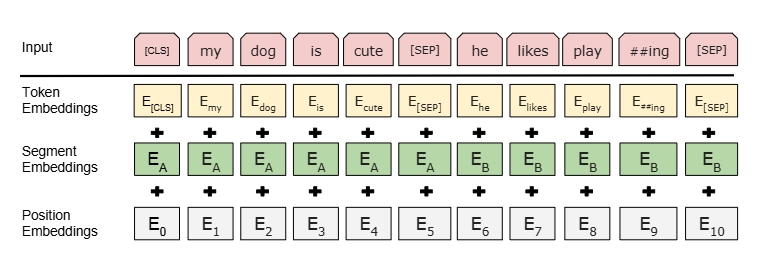
\includegraphics[width=1.0\linewidth]{bert_input.png}
    \caption{Input type of Bert}
    \label{fig:input}
\end{figure}

In Huggingface API, we essentially unpack the dict and directly pass it through the model. But inside it, the 128 dimentions input\_ids are first passed through the Embedding layer along with the position encoding to get the word embedding, the output is of shape 

\begin{center}
 1, 128, 768  
\end{center}

1 is the batch size, 128 is the max\_length, 768 is the internal hidden layer size. 

\begin{figure}[h]
    \centering
    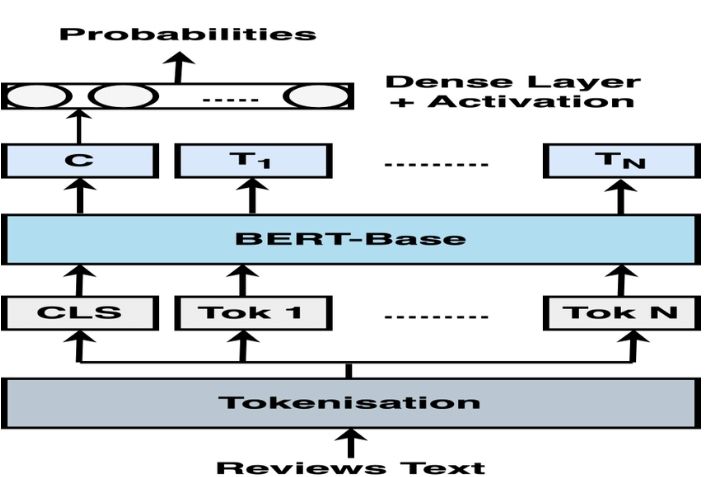
\includegraphics[width=0.8\linewidth]{bert_finetune.png}
    \caption{Bert Classifier}
    \label{fig:model}
\end{figure}


The transformer encoder layer accepts the output of embedding layer. Each encoder consists of Multi-Head Attention and a FF. Also there is residue link. The well known attention is calculated as: 


\[\text{Attention}(Q, K, V) = \text{softmax}\left(\frac{QK^T}{\sqrt{d_k}}\right) V
\]

Finally, the Feed-forward network will give 2 logits. We can get the logits and obtain the label by selecting the larger number given by softmax \[
\text{softmax}(z_i) = \frac{e^{z_i}}{\sum_{j=1}^n e^{z_j}}
\]
After a batch of forward steps, we need to compute the loss function. Here we use 1-accuracy as the loss. \[
\text{Accuracy} = \frac{TP + TN}{TP + TN + FP + FN}
\]
Given that \(\text{Loss} = 1 - \text{Accuracy}\), we can expand it as follows:
\[
\text{Loss} = 1 - \frac{TP + TN}{TP + TN + FP + FN}
\]
Rearranging this, we get:

\[
\text{Loss} = \frac{(TP + TN + FP + FN) - (TP + TN)}{TP + TN + FP + FN}
\]

which simplifies to:
\[
\text{Loss} = \frac{FP + FN}{TP + TN + FP + FN}
\]
\hypertarget{hpd}{{\color{red}{\hyperlink{hhpd}{task d}}}}As for the hyperparameter search strategy, we utilize the optuna. Optuna is a framework-free optimization lib. Since we have no prior knowledge to this specific task for product view, so we simply run many times and try a large space of hyperparameter. Here is code snippet of how to complete the training routine.

\begin{lstlisting}[language=Python, numbers=left]
study = optuna.create_study(direction="maximize")
study.optimize(objective, n_trials=10)

best_params = study.best_params
print(f"Best parameters: {best_params}")
print(f"Best accuracy: {study.best_value}")

final_training_args = TrainingArguments(
    output_dir=os.path.join('checkpoint', FINETUNED),
    learning_rate=best_params["learning_rate"],
    per_device_train_batch_size=best_params["per_device_train_batch_size"],
    num_train_epochs=best_params["num_train_epochs"],
    weight_decay=best_params["weight_decay"],
    save_strategy="epoch",
    evaluation_strategy="epoch"
)
final_model = AutoModelForSequenceClassification.from_pretrained(
    PRETRAIN_HF_NAME, 
    num_labels=2
)

final_trainer = Trainer(
    model=final_model,
    args=final_training_args,
    train_dataset=tokenized_train_dataset,
    eval_dataset=tokenized_test_dataset,
    compute_metrics=compute_metrics,
)

final_trainer.train()
final_eval_result = final_trainer.evaluate()
print(f"Final test accuracy: {final_eval_result['eval_accuracy']}")
final_model_path = os.path.join('checkpoint', FINETUNED, 'my_final_model')
final_trainer.save_model(final_model_path)
tokenizer.save_pretrained(final_model_path)

\end{lstlisting}

\subsection{Analyze Result}

\hypertarget{hpf}{{\color{red}{\hyperlink{hhpf}{task f}}}}We cross validate multiple results from different method, the agreement exceeds 85 percent. After manually check, most of the results make sense. For instance: \\\textit{ Great value for the cost. Fits the iPod well and makes for easy use }\\This is apparently a positive review, and the prediction gives the correct 1.
\\[3mm]But we also find some wrong classified reviews, such as: \textit{My Nike shoes are much better than these shit}\\The model gives positive prediction, which is wrong.
\\[3mm]So we can find that this finetuned encoder model really have a good knowledge of human language, while in some circumstances it cannot understand the real life context and give the wrong prediction. If people deliberately say the opposite, many times humans can distinguish it, but models may not be effective because the same sentence may have completely opposite meanings.




\subsection{Feature Format Discussion}

\hypertarget{hpg}{{\color{red}{\hyperlink{hhpg}{task g}}}}In the most simple TFIDF format, there is only one vector representing the sentence, BOW will always lose much information. Word2Vec and GloVe embedding give each word a vector, provding more information. In transformer encoder based method, each word will have a vector along with its position vector, so the accuracy will be higher than previous methods accuracy. But more information means more resource consumption.

\section{Possible Approaches with Real-word Datasets}
We’ve already trained several models with classic and novel approaches. But in a real-world sentiment analysis task, a perfectly labelled training set cannot be guaranteed. We can break down this challenge into two situations:
\begin{enumerate}
    \item Training set comes partially labelled or doesn’t have rating scores at all.
    \item The training set is labelled with noisy annotations.
\end{enumerate}

\noindent {For the first scenario, we have two ways to tackle the problem:\hypertarget{hph}{{\color{red}{\hyperlink{hhph}{task h}}}}}
\begin{enumerate}
    \item Co-Training: If the training dataset comes partially labelled and samples have two views that are mutually redundant (e.g., a dataset of people where samples are represented by their ID and facial features), two classifiers can be trained on each view and later used to predict the unlabeled subset to augment the labelled one. This method assumes there are two feature dimensions that are mutually uncorrelated, so it is not suitable for our task but worth mentioning {\color{blue}{[23]}}.
    \item Transfer learning with Pre-Trained Models : Pre-trained models like BERT, which have usually been trained on a huge amount of data, have been proven to perform well on none to minimally labeled datasets {\color{blue}{[24]}}.
\end{enumerate}

If the training set is noisily annotated, we also have three approaches:\hypertarget{hpi}{{\color{red}{\hyperlink{hhpi}{task i}}}}
\begin{enumerate}
    \item Loss Function Correction: Adjust the loss function during the training stage to account for noisy labels and thus minimize its effect on the final model. This approach assumes there is a Noise Transition Matrix \( T \) representing the probability of a true label being transformed into another. This matrix can be estimated using a clean noise-free validation set. However, the estimation is often not very effective and far from the genuine one {\color{blue}{[25]}}.
    \item Noise Adaptation Layer: Include a specialized layer within the model architecture that will learn how to adapt and correct for the label noise. This layer is usually a fully connected layer before the final output and will dynamically learn the noise distribution during the training stage. This mechanism is simple yet effective, tackling the problem internally within the model without explicit assumptions {\color{blue}{[26]}}.
    \item Ensemble Methods: Train multiple weaker models that make predictions in parallel and take the majority vote before the final output {\color{blue}{[27]}}.
\end{enumerate}




\bibliographystyle{unsrt}
\begin{thebibliography}{99}  
\bibitem{ref1}Ramos, J., "Using tf-idf to determine word relevance in document queries," Proceedings of the First Instructional Conference on Machine Learning, vol. 242, no. 1, pp. 29–48, 2003, Citeseer.
\bibitem{ref2}T. Mullen and N. Collier, “Sentiment Analysis using Support Vector Machines with Diverse Information Sources,” in Proceedings of the 2004 Conference on Empirical Methods in Natural Language Processing, D. Lin and D. Wu, Eds., Barcelona, Spain: Association for Computational Linguistics, Jul. 2004, pp. 412–418. Accessed: Nov. 13, 2024. [Online]. Available: https://aclanthology.org/W04-3253
\bibitem{ref3}M. Ahmad, S. Aftab, and I. Ali, “Sentiment Analysis of Tweets using SVM,” International Journal of Computer Applications, vol. 177, pp. 975–8887, Nov. 2017, doi: 10.5120/ijca2017915758.
\bibitem{ref4}Y. Al Amrani, M. Lazaar, and K. E. El Kadiri, “Random Forest and Support Vector Machine based Hybrid Approach to Sentiment Analysis,” Procedia Computer Science, vol. 127, pp. 511–520, Jan. 2018, doi: 10.1016/j.procs.2018.01.150.
\bibitem{ref5}M. E. Basiri, S. Nemati, M. Abdar, E. Cambria, and U. R. Acharya, “ABCDM: An Attention-based Bidirectional CNN-RNN Deep Model for sentiment analysis,” Future Generation Computer Systems, vol. 115, pp. 279–294, Feb. 2021, doi: 10.1016/j.future.2020.08.005.
\bibitem{ref6}E. F. Can, A. Ezen-Can, and F. Can, “Multilingual Sentiment Analysis: An RNN-Based Framework for Limited Data,” Jun. 08, 2018, arXiv: arXiv:1806.04511. doi: 10.48550/arXiv.1806.04511.
\bibitem{ref7}Dr. G. S. N. Murthy, Shanmukha Rao Allu, Bhargavi Andhavarapu, Mounika Bagadi, Mounika Belusonti, and Aditya Institute of Technology and Management, “Text based Sentiment Analysis using LSTM,” IJERT, vol. V9, no. 05, p. IJERTV9IS050290, May 2020, doi: 10.17577/IJERTV9IS050290.
\bibitem{ref8}R. K. Behera, M. Jena, S. K. Rath, and S. Misra, “Co-LSTM: Convolutional LSTM model for sentiment analysis in social big data,” Information Processing Management, vol. 58, no. 1, p. 102435, Jan. 2021, doi: 10.1016/j.ipm.2020.102435.
\bibitem{ref9}J. Devlin, M.-W. Chang, K. Lee, and K. Toutanova, “BERT: Pre-training of Deep Bidirectional Transformers for Language Understanding,” May 24, 2019, arXiv: arXiv:1810.04805. Accessed: Nov. 14, 2024. [Online]. Available: http://arxiv.org/abs/1810.04805
\bibitem{ref10}N. Bahrawi, “Sentiment Analysis Using Random Forest Algorithm-Online Social Media Based,” JITU, vol. 2, no. 2, pp. 29–33, 2019, doi: 10.30818/jitu.2.2.2695.
\bibitem{ref11}S. Angel. Deborah, T. T. Mirnalinee, and S. M. Rajendram, “Emotion Analysis on Text Using Multiple Kernel Gaussian...,” Neural Process Lett, vol. 53, no. 2, pp. 1187–1203, Apr. 2021, doi: 10.1007/s11063-021-10436-7.
\bibitem{ref12}I. Roman, A. Mendiburu, R. Santana, and J. A. Lozano, “Sentiment analysis with genetically evolved gaussian kernels,” in Proceedings of the Genetic and Evolutionary Computation Conference, in GECCO ’19. New York, NY, USA: Association for Computing Machinery, Jul. 2019, pp. 1328–1337. doi: 10.1145/3321707.3321779.
\bibitem{ref13}T. Mikolov, I. Sutskever, K. Chen, G. S. Corrado, and J. Dean, "Distributed representations of words and phrases and their compositionality," Advances in Neural Information Processing Systems, vol. 26, 2013.
\bibitem{ref14}A. Joulin, E. Grave, P. Bojanowski, and T. Mikolov, “Bag of Tricks for Efficient Text Classification,” Aug. 09, 2016, arXiv: arXiv:1607.01759. doi: 10.48550/arXiv.1607.01759.
\bibitem{ref15}P. Bojanowski, E. Grave, A. Joulin, and T. Mikolov, “Enriching Word Vectors with Subword Information,” Jun. 19, 2017, arXiv: arXiv:1607.04606. doi: 10.48550/arXiv.1607.04606.
\bibitem{ref16}P. Bojanowski, E. Grave, A. Joulin, and T. Mikolov, “Enriching Word Vectors with Subword Information,” Jun. 19, 2017, arXiv: arXiv:1607.04606. doi: 10.48550/arXiv.1607.04606.
\bibitem{ref17}J. Pennington, R. Socher, and C. Manning, “GloVe: Global Vectors for Word Representation,” in Proceedings of the 2014 Conference on Empirical Methods in Natural Language Processing (EMNLP), A. Moschitti, B. Pang, and W. Daelemans, Eds., Doha, Qatar: Association for Computational Linguistics, Oct. 2014, pp. 1532–1543. doi: 10.3115/v1/D14-1162.
\bibitem{ref18}Y. Liu et al., “RoBERTa: A Robustly Optimized BERT Pretraining Approach,” Jul. 26, 2019, arXiv: arXiv:1907.11692. Accessed: Nov. 14, 2024. [Online]. Available: http://arxiv.org/abs/1907.11692
\bibitem{ref19}V. Sanh, L. Debut, J. Chaumond, and T. Wolf, “DistilBERT, a distilled version of BERT: smaller, faster, cheaper and lighter,” Mar. 01, 2020, arXiv: arXiv:1910.01108. Accessed: Nov. 14, 2024. [Online]. Available: http://arxiv.org/abs/1910.01108
\bibitem{ref20}Z. Ding, Y. Qi, and D. Lin, Albert-based sentiment analysis of movie review. 2021, p. 1246. doi: 10.1109/AEMCSE51986.2021.00254.
\bibitem{ref21}T. B. Brown et al., “Language Models are Few-Shot Learners,” Jul. 22, 2020, arXiv: arXiv:2005.14165. Accessed: Nov. 14, 2024. [Online]. Available: http://arxiv.org/abs/2005.14165
\bibitem{ref22}L. Ouyang, J. Wu, X. Jiang, D. Almeida, C. Wainwright, P. Mishkin, C. Zhang, S. Agarwal, K. Slama, A. Ray, et al., "Training language models to follow instructions with human feedback," Advances in Neural Information Processing Systems, vol. 35, pp. 27730–27744, 2022.
\bibitem{ref23}A. Blum and T. Mitchell, "Combining Labeled and Unlabeled Data with Co-Training," Proceedings of the 11th Annual Conference on Computational Learning Theory, Madison, WI, USA, 1998, pp. 92–100.

\bibitem{ref24}J. Devlin, M.-W. Chang, K. Lee, and K. Toutanova, "BERT: Pre-training of Deep Bidirectional Transformers for Language Understanding," Proceedings of the 2019 Conference of the North American Chapter of the Association for Computational Linguistics: Human Language Technologies, Minneapolis, MN, USA, 2019, pp. 4171–4186.

\bibitem{ref25}G. Patrini, A. Rozza, A. Krishna Menon, R. Nock, and L. Qu, "Making Deep Neural Networks Robust to Label Noise: A Loss Correction Approach," Proceedings of the IEEE Conference on Computer Vision and Pattern Recognition (CVPR), Honolulu, HI, USA, 2017, pp. 2233–2241.

\bibitem{ref26}J. Goldberger and E. Ben-Reuven, "Training Deep Neural-Networks Using a Noise Adaptation Layer," International Conference on Learning Representations (ICLR), Toulon, France, 2017.

\bibitem{ref27}Z.-H. Zhou, Ensemble Methods: Foundations and Algorithms, Boca Raton, FL, USA: Chapman and Hall/CRC, 2012.
\end{thebibliography}

\newpage
\hypertarget{apdxA}{}
\appendixpage
\appendixname{\textbf{\textit{A: Corresponding task and group division of labor}} }


\begin{table}[h]
    \centering
    \begin{tabular}{ |c|c|c| }
         Assignee&  Task& Location in text\\\hline
         Li Siqi&  \textbf{\textit{a.1}}  review in domain& \hypertarget{hhpa.1}{{\color{red}{\hyperlink{hpa.1}{task a.1}}}}\\ 
         Li Siqi&  \textbf{\textit{a.2}}  latest development& \hypertarget{hhpa.2}{{\color{red}{\hyperlink{hpa.2}{task a.2}}}}\\ 
         Li Siqi&  \textbf{\textit{a.3}}  in-depth reading& \hypertarget{hhpa.3}{{\color{red}{\hyperlink{hpa.3}{task a.3}}}}\\ 
         Li Siqi&  \textbf{\textit{a.4}}  combine with task& \hypertarget{hhpa.4}{{\color{red}{\hyperlink{hpa.4}{task a.4}}}}\\ 
         Yang Kaiwen&  \textbf{\textit{b.}}  feature format& \hypertarget{hhpb}{{\color{red}{\hyperlink{hpb}{task b}}}}\\ 
         Yang Kaiwen&  \textbf{\textit{c.}}  build classifier& \hypertarget{hhpc}{{\color{red}{\hyperlink{hpc}{task c}}}}\\ 
         Yang Kaiwen&  \textbf{\textit{d.}}  hyperparameters& \hypertarget{hhpd}{{\color{red}{\hyperlink{hpd}{task d}}}}\\ 
         Yang Kaiwen&  \textbf{\textit{e.}}  prediction& \hypertarget{hhpe}{{\color{red}{\hyperlink{hpe}{task e}}}}\\ 
         Yang Kaiwen&  \textbf{\textit{f.}}  strength/weakness& \hypertarget{hhpf}{{\color{red}{\hyperlink{hpf}{task f}}}}\\ 
         Yang Kaiwen&  \textbf{\textit{g.}}  different feature& \hypertarget{hhpg}{{\color{red}{\hyperlink{hpg}{task g}}}}\\ 
         Zheng Zhikai&  \textbf{\textit{h.}}  unlabeled data& \hypertarget{hhph}{{\color{red}{\hyperlink{hph}{task h}}}}\\ 
         Zheng Zhikai&  \textbf{\textit{i.}}  noisy annotation& \hypertarget{hhpi}{{\color{red}{\hyperlink{hpi}{task i}}}}\\ 
    \end{tabular}
    \caption{Task and assignee}
    \label{tab:my_label1}
\end{table}


\\[10mm]
\appendixname{\textbf{\textit{B: Program Repository}} }
\begin{flushleft}
This project has been hosted in the GitHub repository \url{https://github.com/KuRRe8/Bi-Senti-EE6483}. There is a brief introduction to the use of this repo.

You can either follow the README.md in repo or continue with this page. In the root path of repo, you will find some folders. First you need to install necessary libs instructing in config/requirements.txt. After that you should type \textit{python app.py}, and then you will see the CLI in Figure \ref{fig:AA0}

\begin{figure}[h]
    \centering
    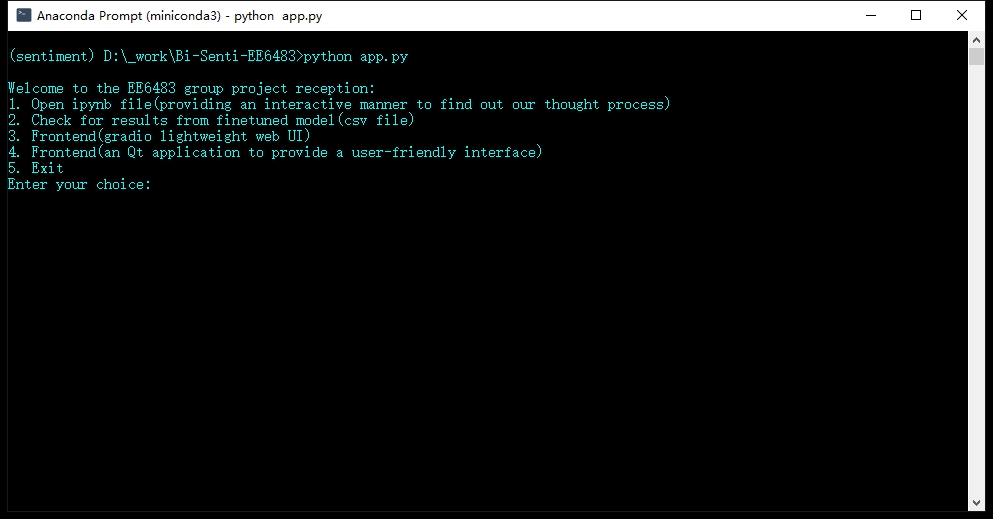
\includegraphics[width=0.9\linewidth]{reception.png}
    \caption{reception}
    \label{fig:AA0}
\end{figure}

select 1 to open the jupyter notebook to experience the whole process of sentiment analysis, including data preprocessing, model training, model evaluation, and model prediction.

\begin{figure}[h]
    \centering
    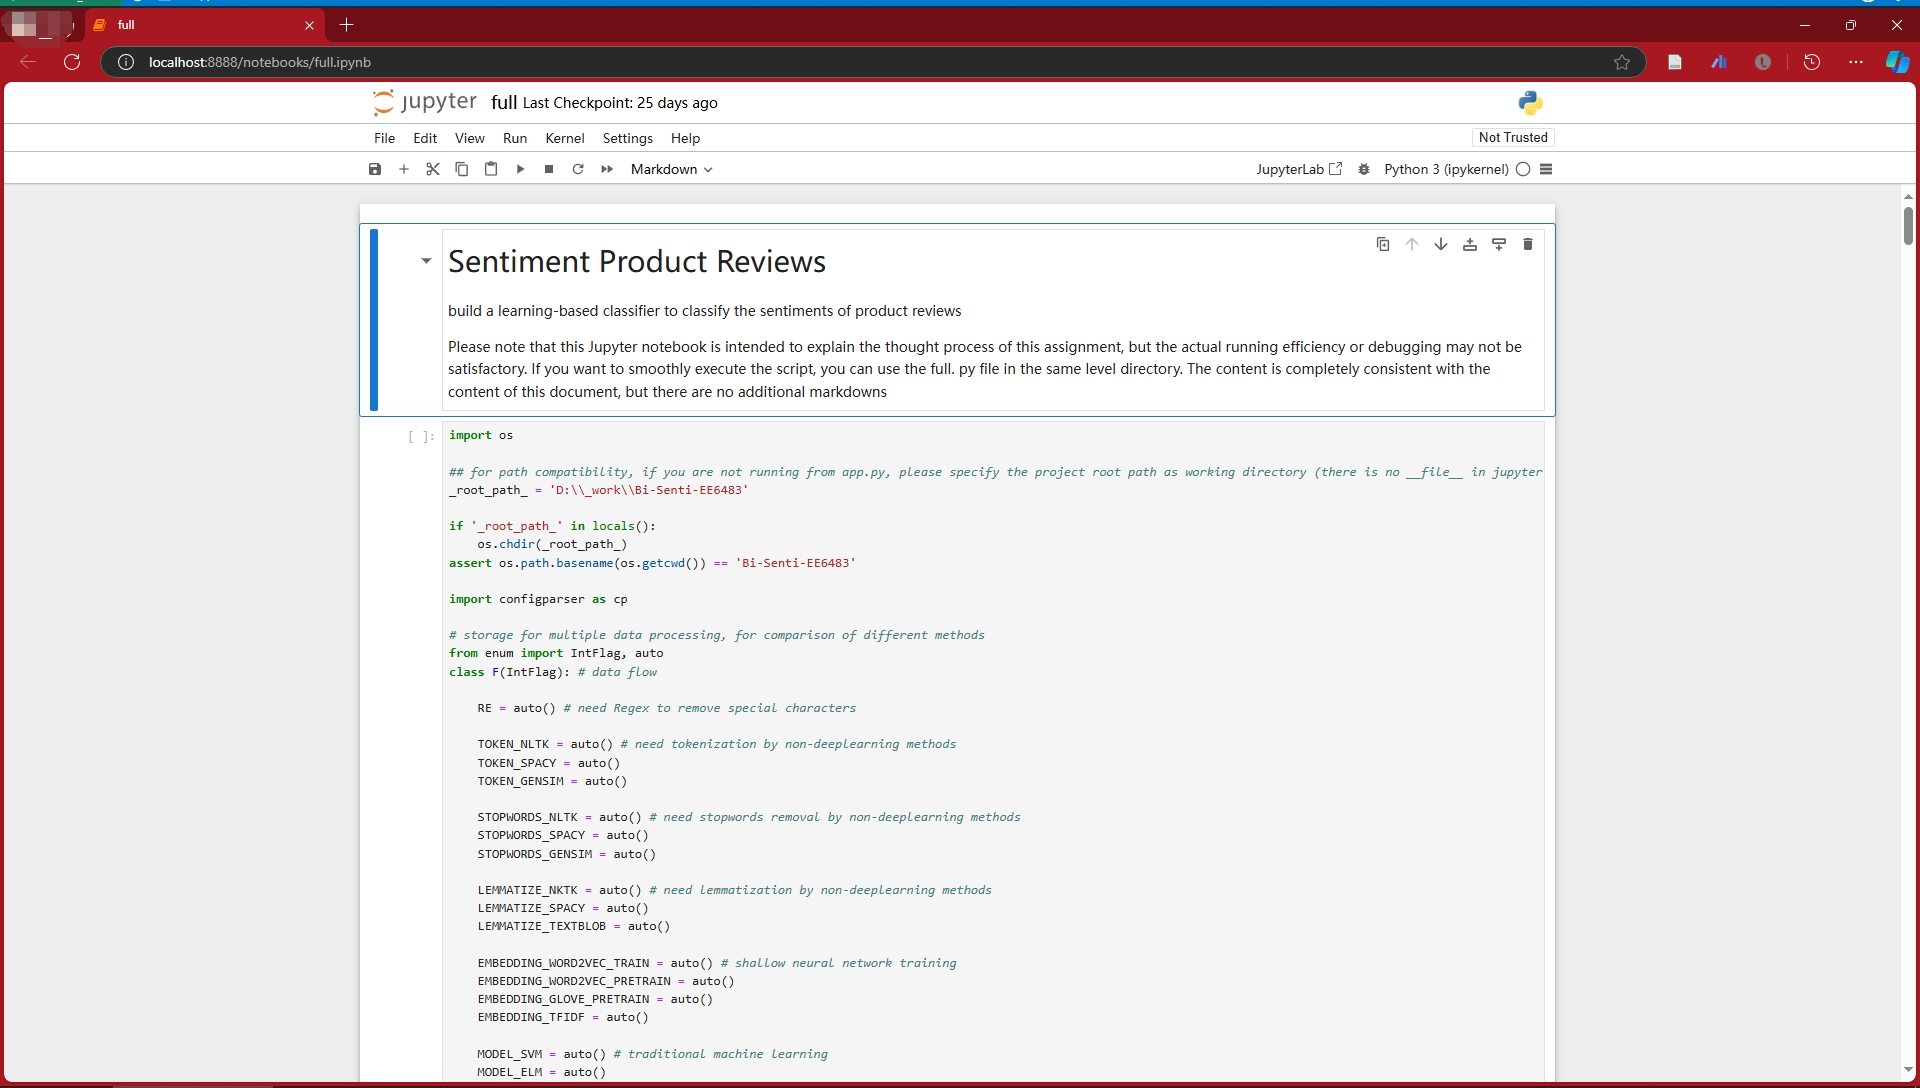
\includegraphics[width=1.0\linewidth]{choice1_jupyter_full_routine_of_nlp.png}
    \caption{Jupyter}
    \label{fig:AA1}
\end{figure}


\textbf{The entire code is segmented based on different functionalities (preprocessing, word embedding, training), rather than segmentation based on the model. The advantage of this approach is that we can freely specify the methods to be used in different stages, achieving high flexibility, and also testing my profound insights into common method process data (especially data shapes)} 

here I already provided 3 task demo. It covers the traditional NLP routines by sci-kit learn and deep learning routines by Pytorch/ Huggingface.

If you just want inference, you can either choose F.ENSEMBLE\_DISTILBERT or other finetuned models as long as the model already exists in the checkpoint folder. Please note that I do not upload the checkpoint on Github. If you have a need of that, please notify me on the discussion panel.

If you choose 2, will give you the file path of our final result csv.
\\[6mm]Choice 3 will start gradio interface for real-time inference.Choice 4 will start Qt frontend. Please note that this needs Pyside2 installed.

\begin{figure}[ht]
    \centering
    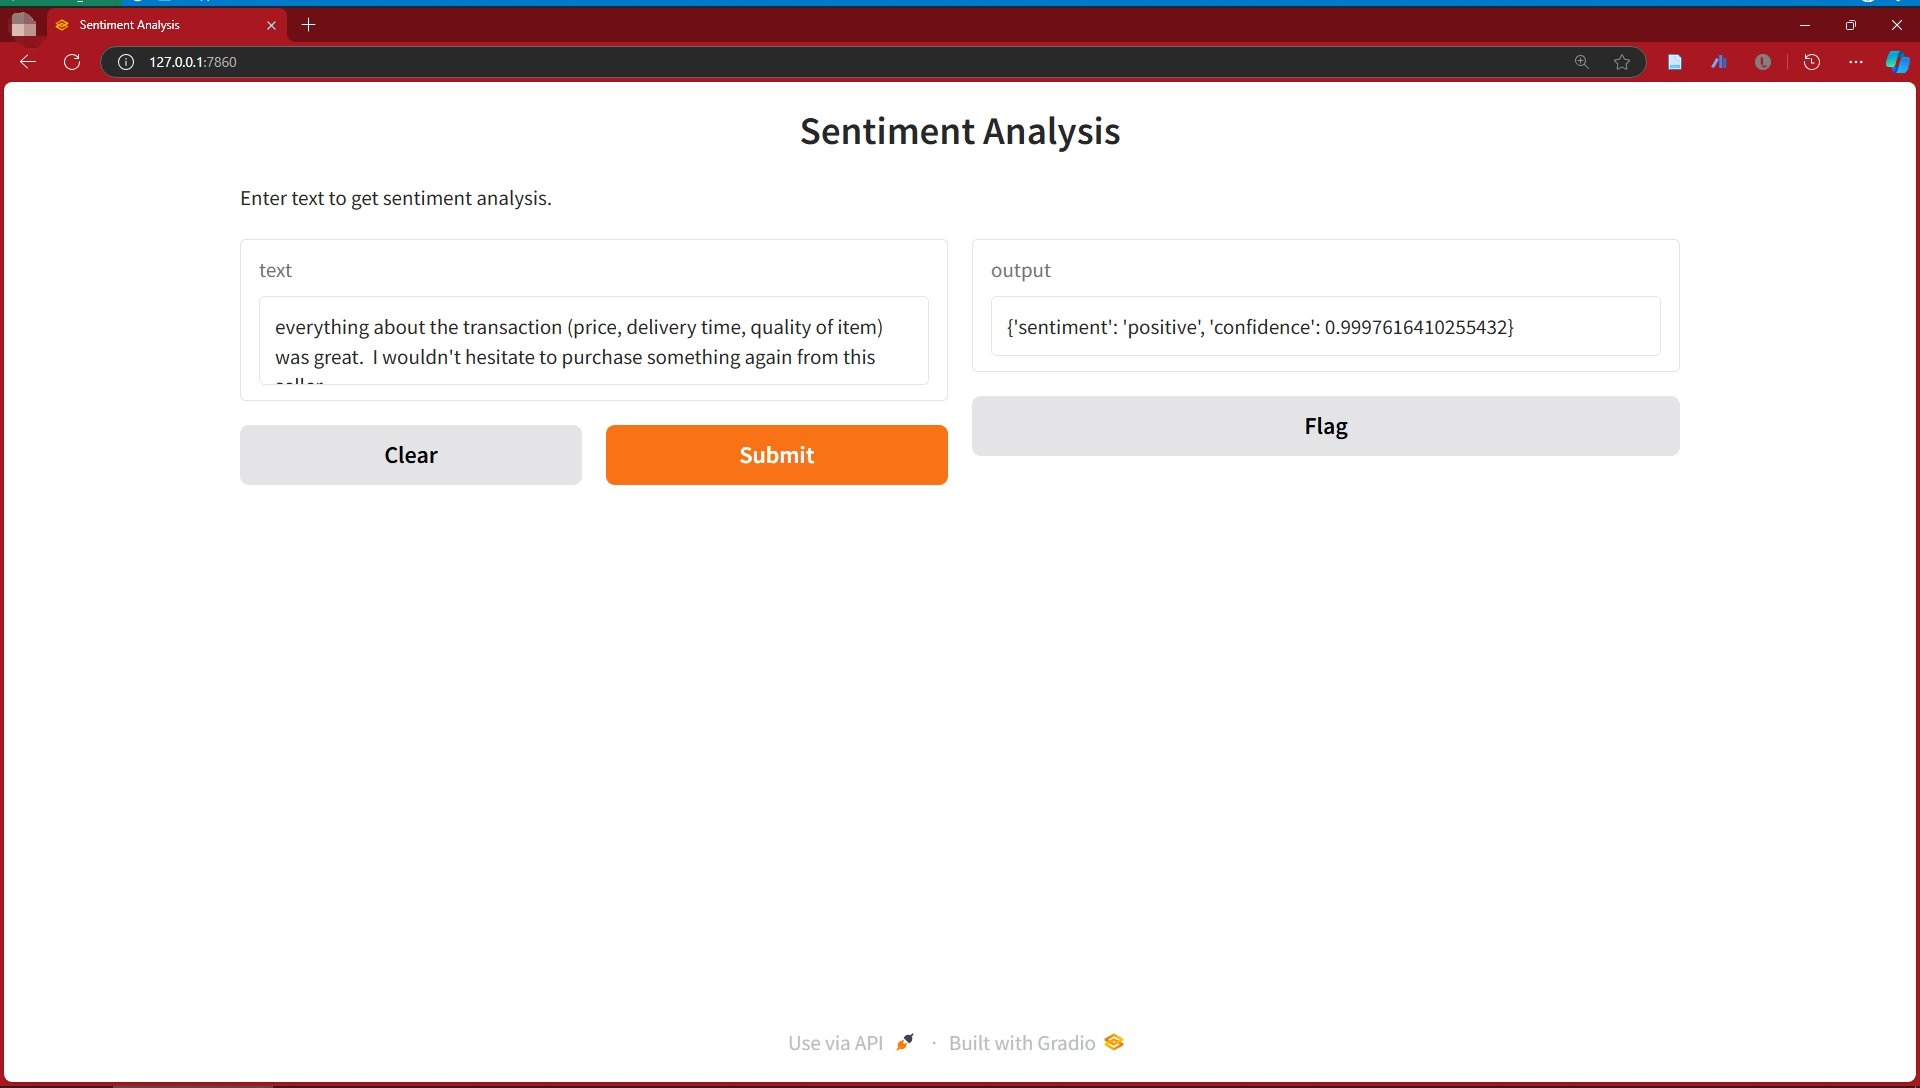
\includegraphics[width=1.0\linewidth]{choice3_gradio_frontend.png}
    \caption{Gradio}
    \label{fig:AA3}
\end{figure}

\begin{figure}[ht]
    \centering
    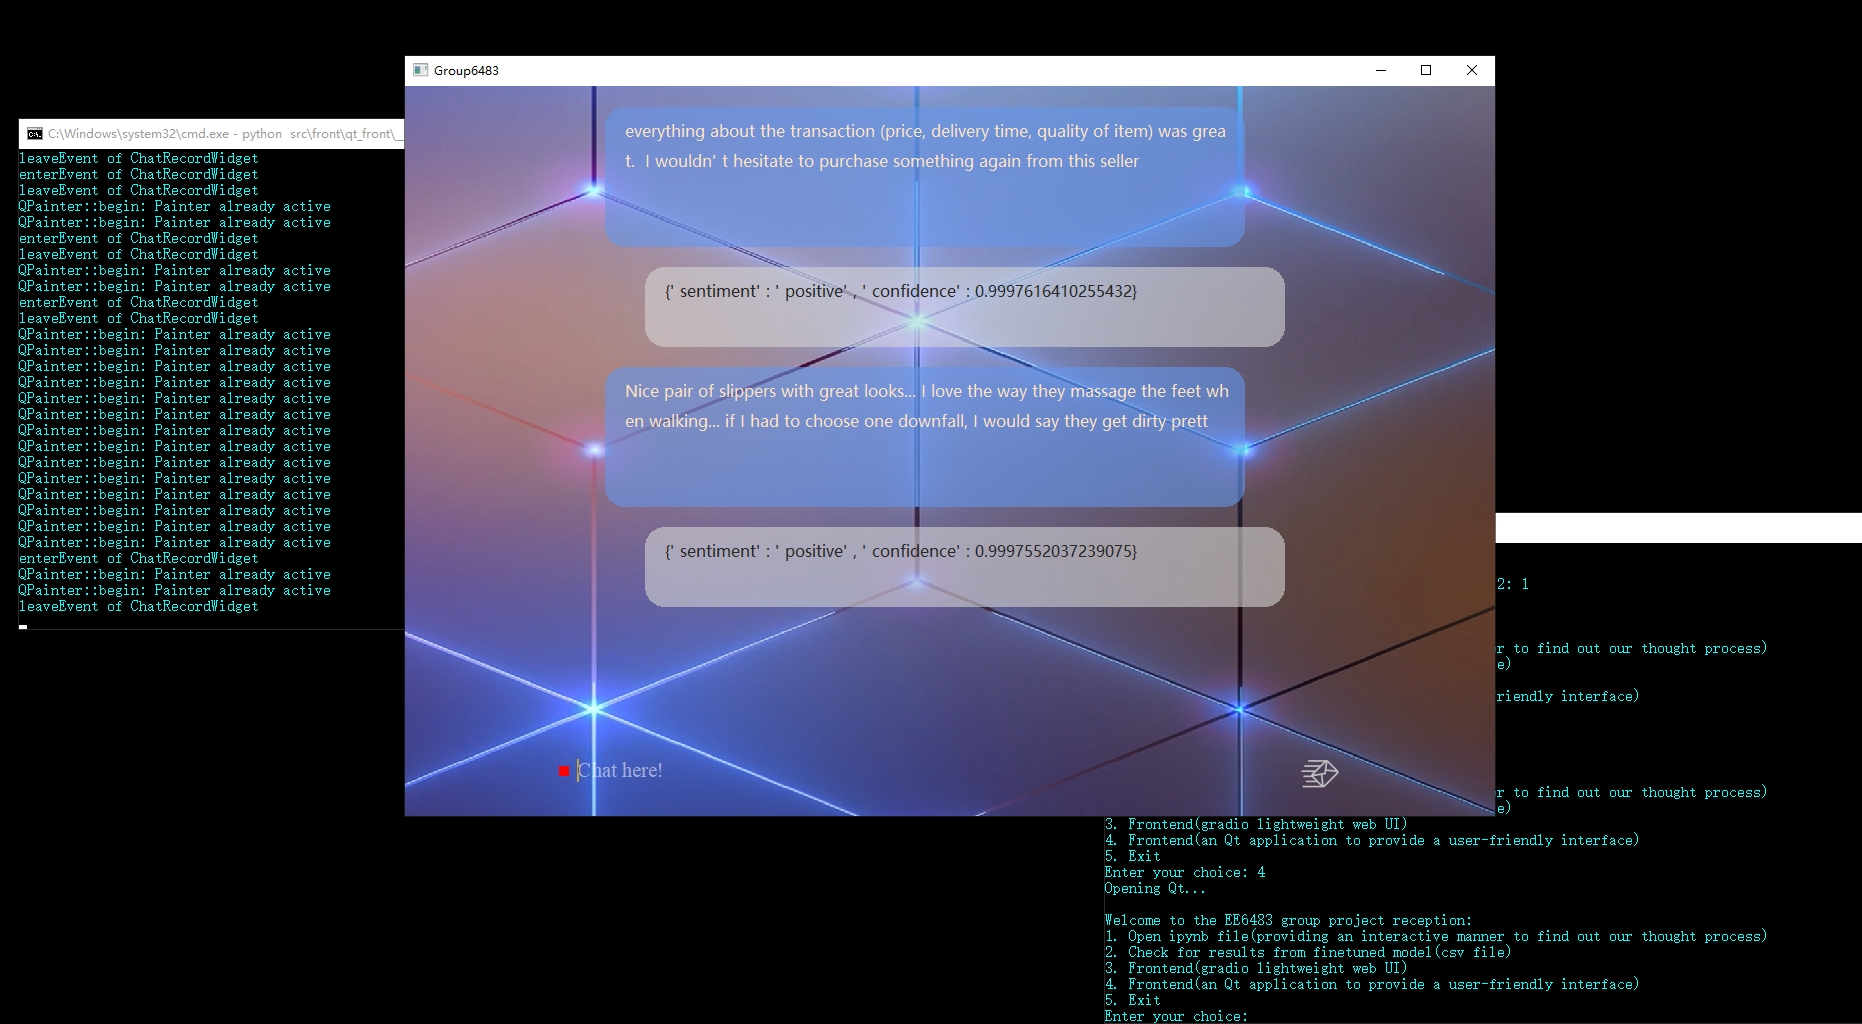
\includegraphics[width=1.0\linewidth]{choice4_qt_frontend.png}
    \caption{Qt}
    \label{fig:AA4}
\end{figure}

\end{flushleft}

\end{document}


